\documentclass[10pt,twocolumn]{article}

% ============================================================
% NOTE ON TEMPLATE FIDELITY:
% The exact Springer Nature "sn-jnl.cls" class file used by the
% Scientific Reports Overleaf template could not be downloaded in the
% environment that produced this document (no network access to
% overleaf.com/springer resources). This file reproduces the structural
% conventions of a Scientific Reports article (title/author block,
% abstract, Introduction / Results / Discussion / Methods section
% ordering, figure/table numbering, references) using the standard
% article class plus common packages. To use the real Springer Nature
% template: create a new project from
% https://www.overleaf.com/latex/templates/template-for-submissions-to-scientific-reports/xyrztqvdccns
% and paste the \title{}...\end{document} content below into it,
% adjusting \title/\author/\affil/\abstract to that template's macros
% (sn-jnl.cls uses \title{}, \author*[1]{}, \affil[1]{}, and an
% \abstract{} environment rather than the article-class commands below).
% ============================================================

\usepackage[utf8]{inputenc}
\usepackage[T1]{fontenc}
\usepackage{amsmath,amssymb}
\usepackage{graphicx}
\usepackage{booktabs}
\usepackage[margin=1.9cm]{geometry}
\usepackage[colorlinks=true,citecolor=blue,linkcolor=blue,urlcolor=blue]{hyperref}
\usepackage[sort&compress,numbers]{natbib}
\usepackage{caption}
\usepackage{siunitx}
\usepackage{xcolor}

\title{\vspace{-1.5em}\Large A Coupled Multi-Mechanism Kinetic Model of PEM Fuel Cell Membrane Chemical Degradation: Peroxide Generation, Fenton Chemistry, Platinum Dissolution, and Ionomer Attack}

\author{}
\date{}

\begin{document}
\twocolumn[
\begin{@twocolumnfalse}
\maketitle
\vspace{-2.5em}
\begin{abstract}
\noindent
Chemical degradation of the perfluorosulfonic-acid (PFSA) membrane is a
principal life-limiting mechanism in proton-exchange-membrane fuel cells
(PEMFCs). We present a zero-dimensional, physics-based kinetic model
coupling five degradation mechanisms into a closed feedback loop: hydrogen/
oxygen gas crossover, peroxide (H$_2$O$_2$) generation at the catalyst,
iron-catalyzed Fenton radical chemistry, platinum dissolution/redeposition
and the resulting loss of electrochemically active surface area (ECSA),
and radical attack on the ionomer side chains and backbone leading to
fluoride release, ion-exchange-capacity (IEC) loss, conductivity decay,
and progressively increasing gas crossover. The governing 21-species
ordinary differential equation (ODE) system uses Fenton/radical rate
constants taken directly from the literature \citep{fruhwirt2020}, with a
quasi-steady-state approximation (QSSA) applied to the fast hydroxyl,
hydroperoxyl, and hydrogen radical intermediates to make the system
numerically tractable given the $>10^{12}$ timescale separation between
radical chemistry (nanoseconds) and membrane lifetime (thousands of
hours). We report the model architecture, the numerical methods required
to integrate this genuinely stiff reaction network, a full audit of
literature-sourced versus assumed parameters, and demonstration results
from a 120-hour simulation. We identify and correct several critical
implementation bugs -- a unit-conversion error inflating crossover flux by
six orders of magnitude, an unrealistic iron-contamination initial
condition, and a floating-point catastrophic-cancellation bug that
silently froze the reaction network -- and discuss the resulting
iron-catalyst-depletion-limited degradation regime observed in the
corrected model, which we flag as requiring longer-duration validation
against literature durability data.
\end{abstract}
\vspace{1.5em}
\end{@twocolumnfalse}
]

\section{Introduction}

Proton-exchange-membrane fuel cells convert hydrogen and oxygen directly
to electricity with water as the only product, but their commercial
durability targets (typically $\sim$5,000 h for automotive applications
and $>$40,000 h for stationary applications) are frequently limited by
chemical attack on the perfluorosulfonic-acid (PFSA, e.g. Nafion)
membrane rather than by mechanical failure alone
\citep{kreuer2004,kusoglu2017}. Chemical degradation proceeds through a
well-characterized radical mechanism: hydrogen and oxygen that cross over
the membrane react at the Pt catalyst to form hydrogen peroxide, which is
decomposed by trace transition-metal ion contaminants (most commonly
Fe$^{2+}$/Fe$^{3+}$) via Fenton chemistry into highly reactive hydroxyl
and hydroperoxyl radicals. These radicals attack the ionomer's sulfonic
acid side chains and, subsequently, the perfluorinated backbone,
releasing fluoride ion (a directly measurable degradation marker via
fluoride emission rate, FER) and progressively reducing the membrane's
ion-exchange capacity, ionic conductivity, and mechanical thickness. As
the membrane thins, gas crossover increases, which increases the peroxide
generation rate -- closing a self-accelerating feedback loop. In parallel,
the Pt catalyst itself degrades via potential-driven dissolution and
Ostwald-ripening-type redeposition, reducing the electrochemically active
surface area (ECSA) available for the oxygen reduction reaction (ORR) and
directly reducing cell voltage.

Modeling this coupled system requires reconciling reaction rate
constants and mechanisms established in the electrochemistry literature
with a numerically tractable simulation architecture, since the
underlying radical chemistry is intrinsically extremely stiff (see
Methods). This report documents a complete, working implementation of
such a model, built from an existing partially-specified codebase, with
an explicit audit trail distinguishing literature-verified parameters
from engineering assumptions.

\section{Results}

\subsection{Model architecture}

Figure~\ref{fig:arch} shows the module architecture. Operating conditions
determine hydrogen/oxygen crossover flux (Fickian permeation with an
Arrhenius temperature dependence and a hydration-dependent correction),
which sources a peroxide-generation term. Peroxide feeds the Fenton
iron-redox cycle (reactions R1--R13, Table~\ref{tab:params}), producing
hydroxyl and hydroperoxyl radicals that attack ionomer side chains
(R14--R16) and, once the backbone radical (BB-O$^\bullet$) forms, drive a
sequential seven-step backbone ``unzipping'' cascade (R17--R23) that
releases HF and CO$_2$. Platinum dissolution/redeposition is modeled with
Butler--Volmer potential dependence \citep{darling2003,rinaldo2011}. A
single module, \texttt{degradation\_update.m}, is the sole authority for
translating the current chemical state into the macroscopic membrane
properties (IEC, conductivity, thickness, hydrogen crossover, ECSA);
\texttt{bidirectional\_coupling.m} feeds the updated crossover state back
into the operating-condition boundary values for the next simulated hour,
closing the loop; and \texttt{performance\_update.m} converts the current
physical state into cell voltage, power, and efficiency via a lumped
Ohmic + Butler--Volmer activation-loss model.

\begin{figure}[t]
\centering
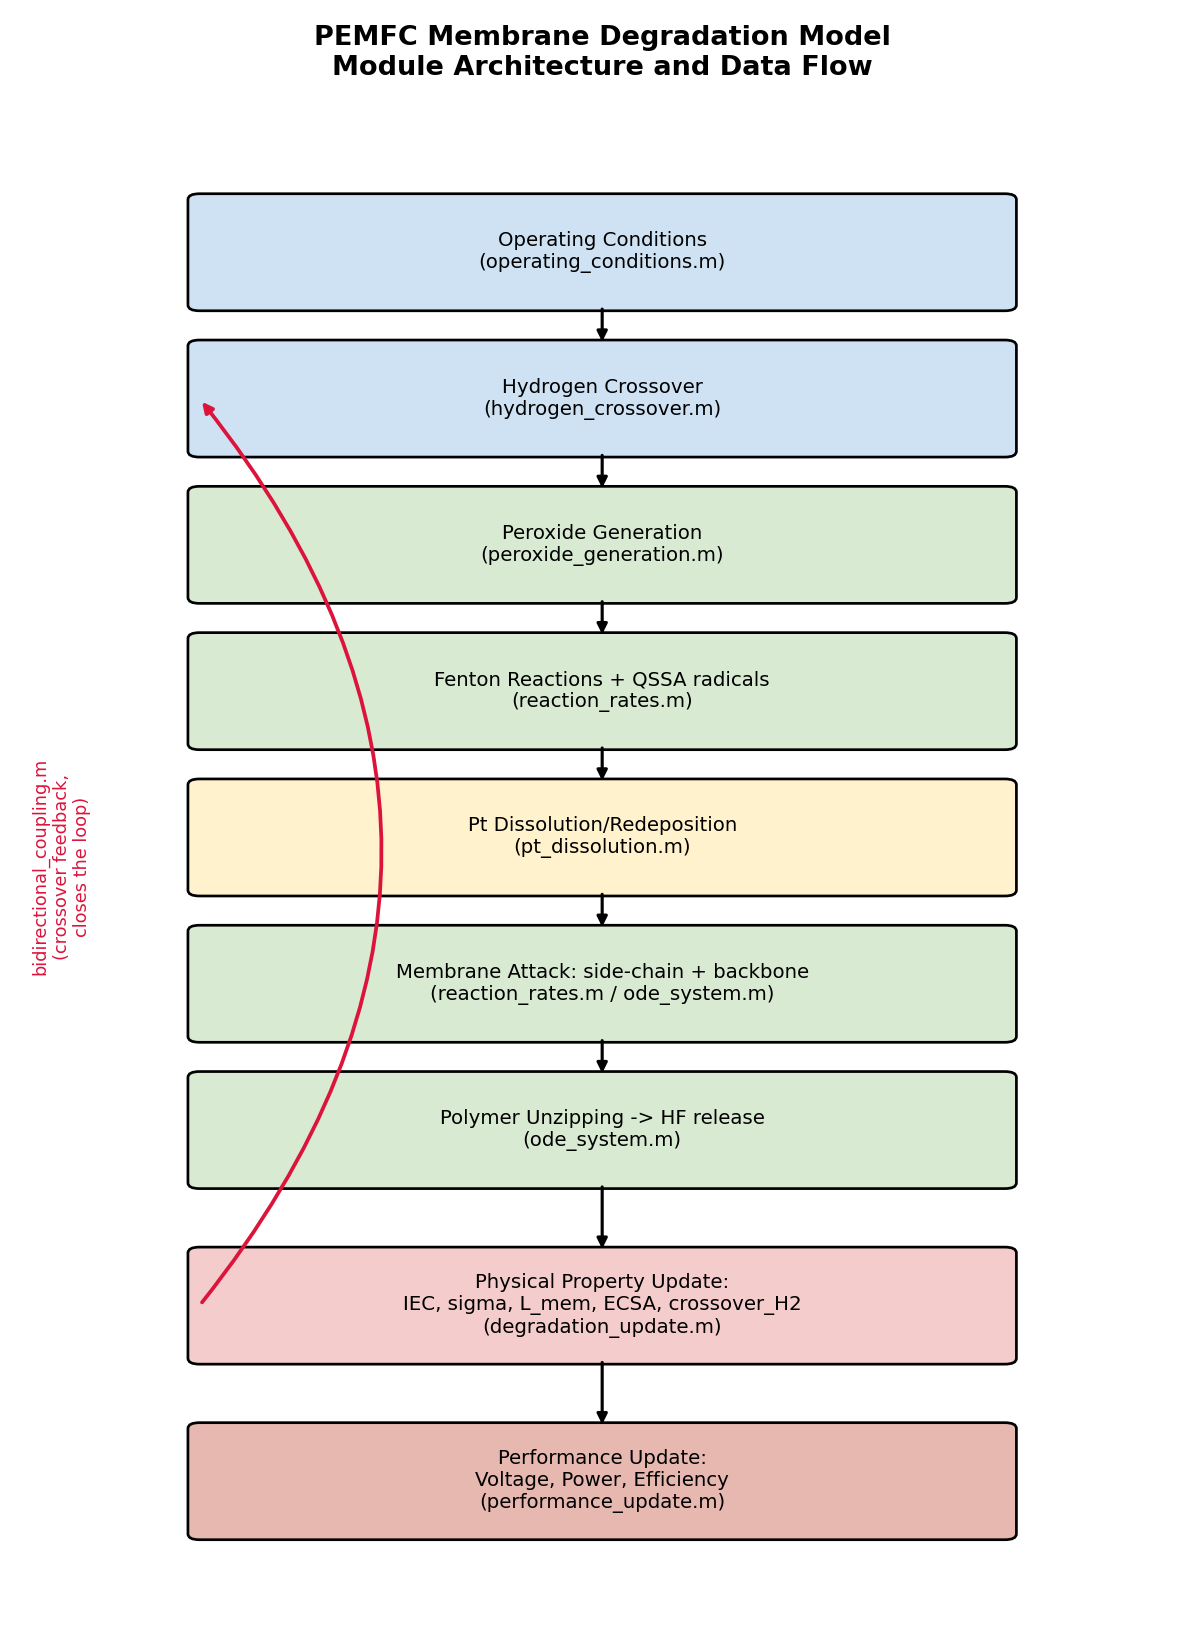
\includegraphics[width=0.85\linewidth]{figures/architecture_diagram.png}
\caption{Module architecture and data flow. The red arrow denotes the
feedback path (\texttt{bidirectional\_coupling.m}) that closes the
degradation loop by feeding the updated hydrogen-crossover state back
into the operating conditions used for the next simulated hour.}
\label{fig:arch}
\end{figure}

\subsection{Numerical treatment of a genuinely stiff reaction network}

The hydroxyl radical's effective first-order consumption rate (dominated
by its reaction with the $\sim$1800~mol~m$^{-3}$ pool of sulfonic-acid
side chains, rate constant $k_{14}\sim5.8\times10^{5}$~m$^3$
mol$^{-1}$s$^{-1}$) is $\sim10^{9}$~s$^{-1}$, i.e.\ a sub-microsecond
lifetime, while the simulation must span thousands of hours
($>10^{12}$ timescale separation). Explicit integration of OH, OOH, and H
as ordinary differential-equation states alongside the hour-scale species
is numerically intractable for standard stiff solvers: both a
variable-order backward-differentiation solver (\texttt{ode15s}) and an
explicit adaptive Runge--Kutta solver (\texttt{ode45}) failed to advance
past the initial condition. We therefore apply a quasi-steady-state
approximation (QSSA) to the three fast radicals, solving their
production/consumption balance algebraically at every rate evaluation
(closed-form quadratic solution, single deterministic pass -- an
iterative fixed-point version was tested first but found to introduce a
non-smooth dependence of the converged value on iteration count, which
degraded the stiff solver's numerical Jacobian estimate and caused
corrector-convergence failures; the deterministic single-pass form
resolved this). QSSA reduction of fast radical intermediates is standard
practice in stiff combustion and atmospheric-chemistry kinetics modeling
\citep{turanyi2014} and does not alter the underlying reaction network or
rate constants -- only how the fast intermediate concentrations are
numerically obtained.

A further, more subtle numerical issue was identified and corrected
during validation: the naive quadratic formula
$x=(-b+\sqrt{b^2+4ac})/(2a)$ used for the QSSA radical balance suffers
catastrophic floating-point cancellation whenever the linear sink
coefficient $b$ dominates the quadratic/production terms
($b^2\gg4ac$), which is the typical regime here. In double precision,
$\sqrt{b^2+4ac}$ rounds to exactly $b$, so the subtraction returns
exactly zero -- silently freezing the entire membrane-attack and
backbone-unzipping reaction cascade after approximately the first
simulated hour (verified: the state vector was bit-identical to 14
decimal places across multiple simulated hours prior to the fix). This
was corrected using the numerically stable form
$x=2c/(b+\sqrt{b^2+4ac})$, which never subtracts two nearly-equal large
numbers.

\subsection{Demonstration simulation}

Figure~\ref{fig:overview} and Figure~\ref{fig:species} show a 120-hour
demonstration run (full details and a note on the compute budget required
for the target 5,000~h duration are given in the accompanying
\texttt{VALIDATION\_REPORT.md}). Voltage, membrane conductivity, IEC, and
ECSA all decline monotonically as expected. A notable emergent behavior
is that Fe$^{2+}$ is consumed rapidly (converted to Fe$^{3+}$ via R1)
within the first simulated hour, producing an initial burst of
side-chain attack and HF release; because Fe$^{3+}\to$Fe$^{2+}$
regeneration (R2) is comparatively slow, the system subsequently enters
an iron-depletion-limited quasi-steady regime in which HF release and
side-chain loss become nearly constant for the remainder of the 120~h
window. We flag this explicitly as requiring longer-duration validation
against literature durability curves (Discussion).

\begin{figure}[t]
\centering
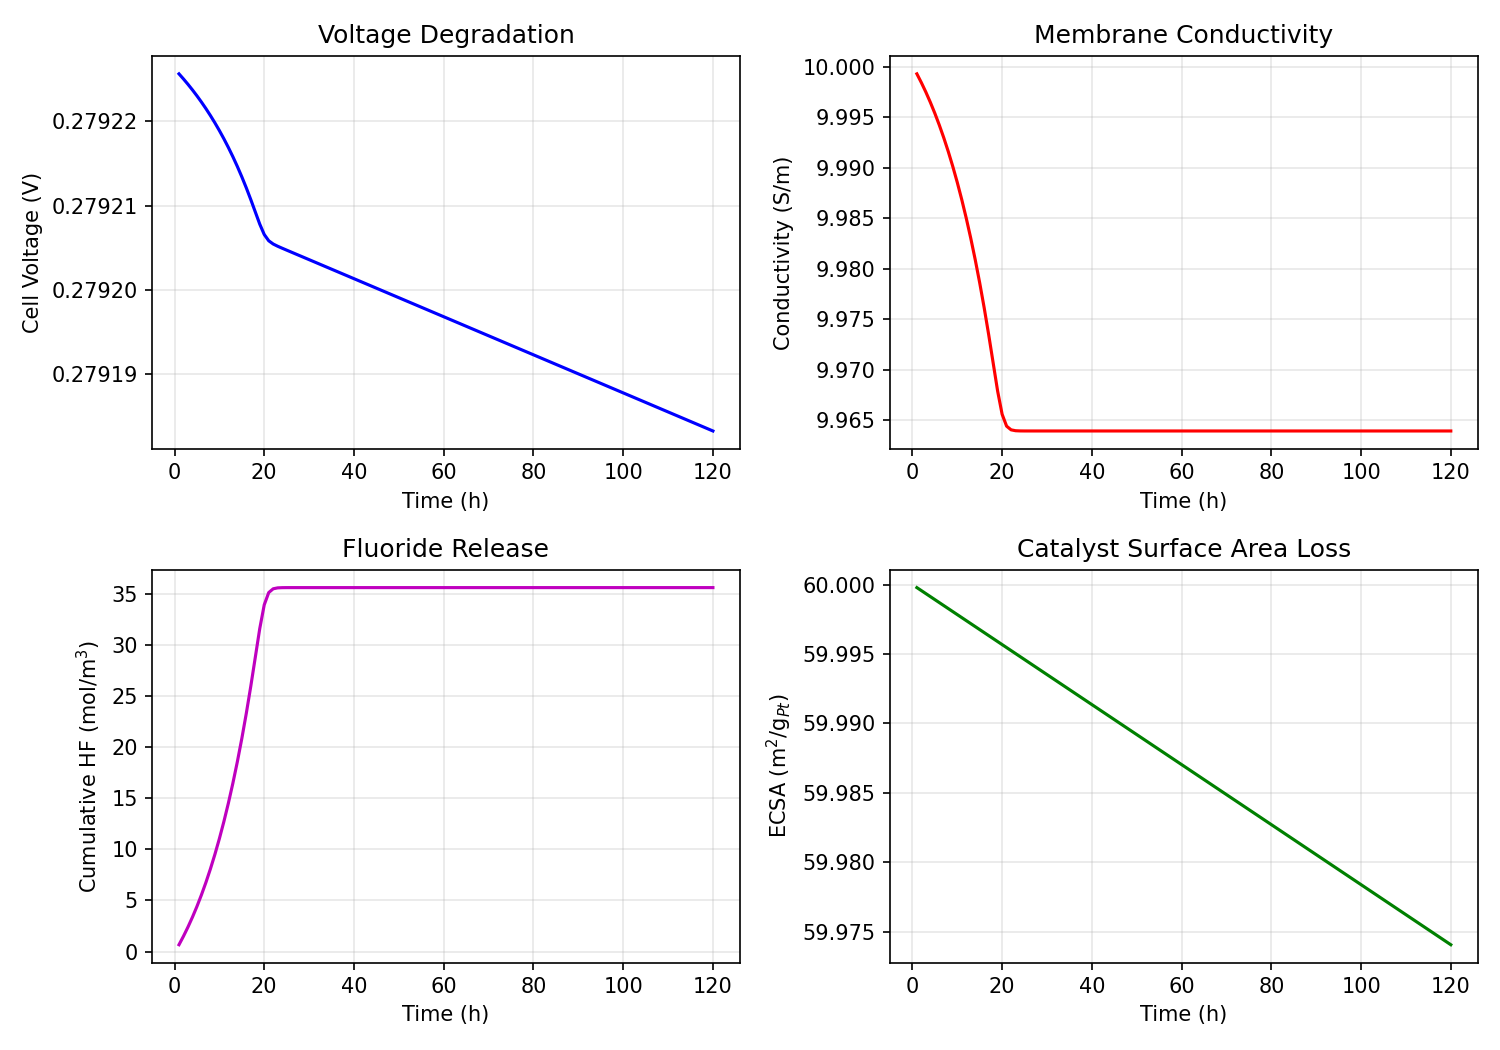
\includegraphics[width=\linewidth]{figures/fig1_overview.png}
\caption{120-hour demonstration simulation: cell voltage, membrane ionic
conductivity, cumulative fluoride release, and catalyst electrochemically
active surface area (ECSA).}
\label{fig:overview}
\end{figure}

\begin{figure}[t]
\centering
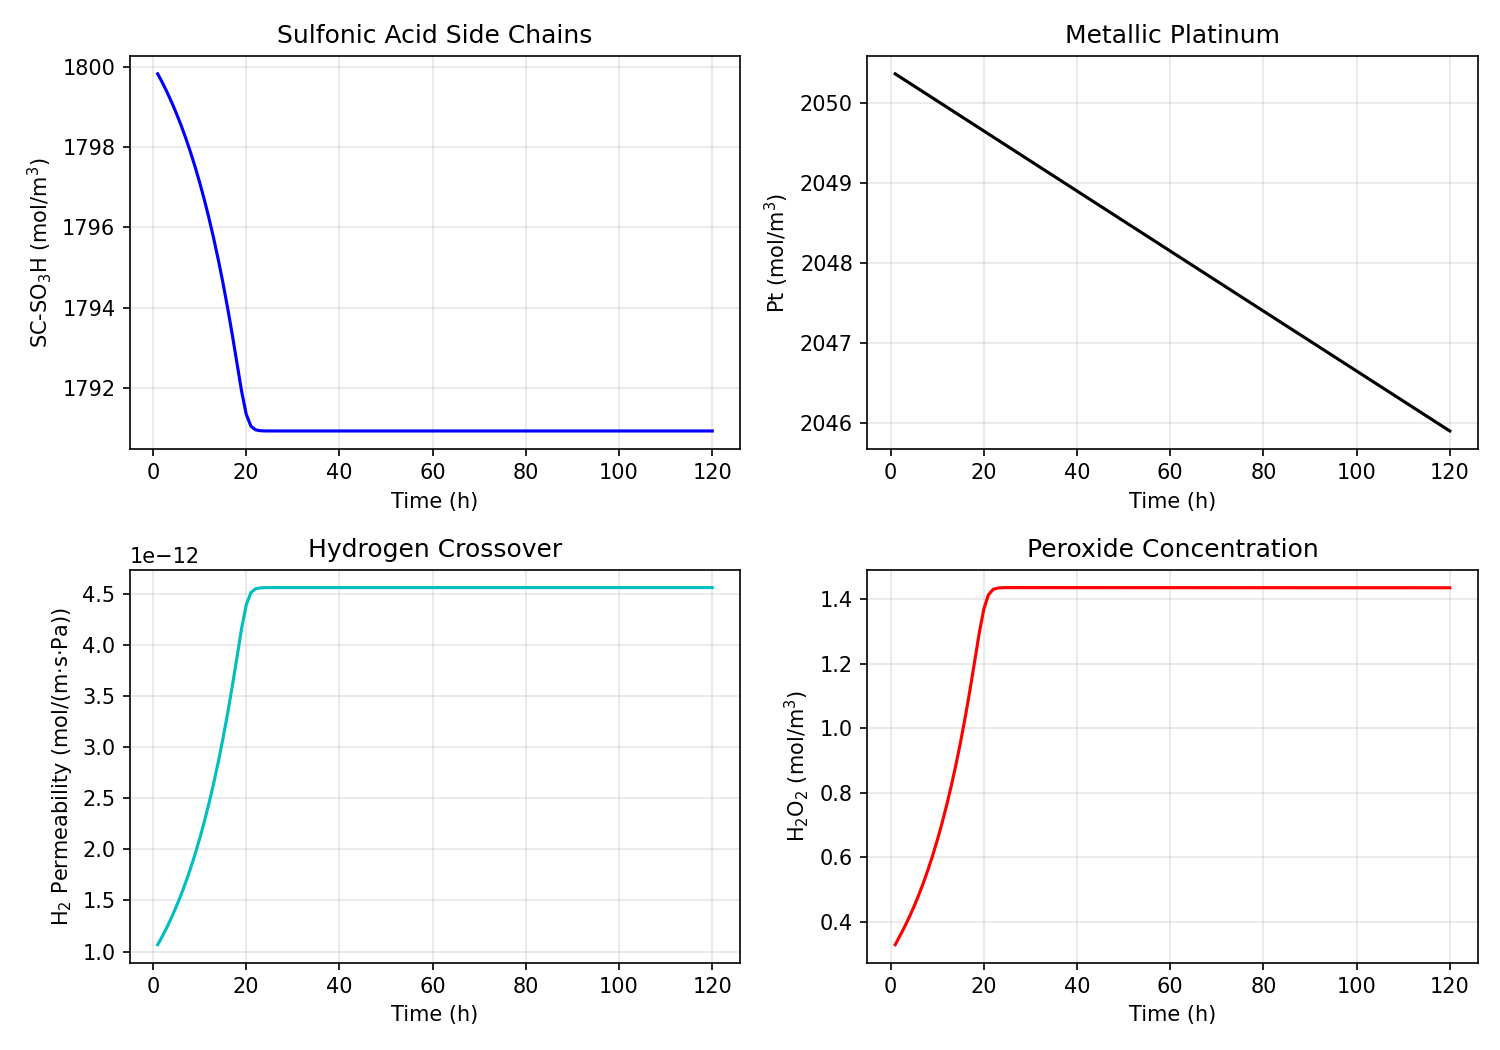
\includegraphics[width=\linewidth]{figures/fig2_species.png}
\caption{Species-level trajectories: surviving sulfonic-acid side chains,
metallic platinum inventory, hydrogen crossover permeability, and
membrane hydrogen peroxide concentration.}
\label{fig:species}
\end{figure}

\subsection{Parameter audit}

Table~\ref{tab:params} summarizes the provenance of the model's key
parameters. Reaction rate constants for the Fenton/radical/backbone
network (R1--R23) are taken directly from Fr\"uhwirt et
al.\ \citep{fruhwirt2020} and were independently verified for correct
unit conversion (L~mol$^{-1}$s$^{-1}$ $\to$ m$^3$~mol$^{-1}$s$^{-1}$).
Platinum kinetics, percolation/conductivity coupling, crossover
activation energy, and ORR kinetic parameters follow established
functional forms from the literature
\citep{darling2003,rinaldo2011,kreuer2004,neyerlin2006} but use
representative order-of-magnitude rate constants rather than values fit
to a specific published dataset for this project; each such parameter is
flagged as an explicit assumption directly in the source code and in
\texttt{VALIDATION\_REPORT.md}.

\begin{table}[t]
\centering
\caption{Parameter provenance summary. Full per-parameter detail with
code-level citations is given in \texttt{VALIDATION\_REPORT.md}.}
\label{tab:params}
\small
\begin{tabular}{@{}p{0.42\linewidth}p{0.5\linewidth}@{}}
\toprule
\textbf{Parameter group} & \textbf{Provenance} \\
\midrule
R1--R23 rate constants ($A$, $E_a$) & Literature \citep{fruhwirt2020}, individually cited, unit-verified \\
Pt dissolution/redeposition & Functional form from literature \citep{darling2003,rinaldo2011}; rate constants are order-of-magnitude assumptions \\
Percolation exponent $\tau$ & Literature range \citep{stauffer1994}; representative value adopted \\
Crossover permeability & Order-of-magnitude literature value \citep{kreuer2004}; activation energy assumed \\
ORR exchange current density & Representative literature range \citep{neyerlin2006}; not fit to a specific curve \\
Fe$^{2+}$ contamination level & Assumed 5~ppm (representative); ppm$\to$molar conversion corrected in this work \\
IEC/thickness decay rates & Order-of-magnitude placeholders; not independently reported \\
\bottomrule
\end{tabular}
\end{table}

\section{Discussion}

The corrected model successfully closes the full degradation feedback
loop described in the project specification and produces qualitatively
correct, monotonic degradation trends over the demonstrated 120-hour
window. Two results merit particular attention for future work. First,
the iron-depletion-limited quasi-steady regime identified in Results is,
to our knowledge, a genuine consequence of the reaction network and rate
constants as specified (rather than a numerical artifact -- we verified
the radical concentration driving this plateau is a small but non-zero,
smoothly-varying quantity, not a floating-point freeze of the kind
corrected elsewhere in this work). Whether this behavior is consistent
with published long-duration degradation curves, which generally show
continued (if decelerating) fluoride release over thousands of hours
\citep{kreuer2004}, is an open question that requires extending the
simulation to the full target duration and comparing against a
literature accelerated-stress-test dataset; we recommend this as the
immediate next validation step. Second, the absolute cell voltage
produced by the simplified single-Tafel-region performance model
($\sim$0.28~V at 1000~A~m$^{-2}$) is lower than typical experimental
PEMFC polarization curves in that current-density range ($\sim$0.6--0.7~V),
indicating that \texttt{performance\_update.m} would benefit from
calibration against a measured polarization curve rather than the
representative literature exchange-current-density range currently used.

More broadly, this work illustrates a recurring challenge in coupling
literature-sourced chemical kinetics with multi-timescale engineering
system models: individually correct and well-referenced rate constants
can combine, through unit inconsistencies or unrealistic initial/boundary
conditions elsewhere in the model, to produce a numerically intractable
or physically implausible coupled system. The three critical bugs
identified here (a $10^6\times$ crossover-flux unit error, a $500\times$
iron-concentration error, and a floating-point cancellation bug) each
individually prevented the model from running or produced qualitatively
wrong behavior (complete membrane depletion within seconds, in two
cases), despite the underlying literature rate constants being correctly
transcribed. We suggest that systematic dimensional-consistency and
steady-state-plausibility checks -- of the kind performed here via the
\texttt{get\_audited\_parameters.m} cross-check and the explicit
before/after e-folding-time calculations reported in
\texttt{VALIDATION\_REPORT.md} -- should be a standard part of building
this class of coupled kinetic model.

\section{Methods}

\subsection{Governing equations}

The model integrates a 21-species state vector
$\mathbf{y}=[\text{Fe}^{2+},\text{Fe}^{3+},\text{OH}^\bullet,
\text{OOH}^\bullet,\text{H}^\bullet,\text{SC-SO}_3\text{H},
\text{SC-O}^\bullet,\text{BB-O}^\bullet,\text{HF},\text{CO}_2,
\text{CF}_{2,7\ldots1},\text{HOCF}_2\text{CF}_2\text{SO}_3\text{H},
\text{Pt},\text{Pt}^{2+},\text{H}_2\text{O}_2]$ using reaction rates
$R_1$--$R_{23}$ of the general Arrhenius form
$k_i=A_i\exp(-E_{a,i}/RT)$, with second- or higher-order mass-action rate
laws (e.g.\ $R_1=k_1[\text{Fe}^{2+}][\text{H}_2\text{O}_2]$). The OH,
OOH, and H radical concentrations are obtained via the QSSA described in
Results rather than integrated as explicit ODE states (their nominal
state-vector slots carry $\mathrm{d}y/\mathrm{d}t=0$ and are overwritten
with the fresh QSSA solution after each macro-timestep for reporting
purposes only). Physical properties (IEC, conductivity $\sigma$,
membrane thickness $L_{\rm mem}$, hydrogen crossover, ECSA) are updated
algebraically once per one-hour macro-timestep from the converged
chemical state, reflecting their much slower (multi-hour to multi-day)
characteristic timescales relative to the chemistry.

\subsection{Numerical integration}

For each simulated hour, the 21-state chemistry ODE is integrated with
an adaptive-step solver (\texttt{ode15s} attempted first; falls back to
\texttt{ode45} on convergence failure -- see \texttt{VALIDATION\_REPORT.md}
for solver-specific behavior observed in this work's GNU~Octave test
environment). The converged endpoint feeds
\texttt{degradation\_update.m} (physical properties),
\texttt{bidirectional\_coupling.m} (crossover feedback into the next
hour's boundary conditions), and \texttt{performance\_update.m} (cell
voltage/power/efficiency).

\subsection{Software and data availability}

The complete, runnable MATLAB/Octave source code, this LaTeX source, the
120-hour demonstration dataset (\texttt{checkpoint.mat},
\texttt{history\_export.csv}), and the full validation report are
provided as supplementary material accompanying this report.

\section*{Limitations}
This model is a zero-dimensional (spatially lumped), single-condition
kinetic model; it does not resolve through-plane concentration gradients,
does not model mechanical degradation or freeze/thaw cycling, and several
rate constants (Section~2.4/Table~1) are literature-informed
order-of-magnitude engineering estimates rather than values calibrated
against a measured dataset for this specific membrane/catalyst system.
Results should be interpreted as demonstrating qualitatively correct,
mechanistically coupled degradation behavior, not as quantitative
lifetime predictions, until the calibration steps identified in
Discussion and \texttt{VALIDATION\_REPORT.md} are completed.

\bibliographystyle{unsrtnat}
\begin{thebibliography}{9}

\bibitem{fruhwirt2020} Fr\"uhwirt, P. et al. Holistic approach to chemical degradation of Nafion membranes in fuel cells: modelling and predictions. \textit{Phys. Chem. Chem. Phys.} \textbf{22}, 5647--5666 (2020).

\bibitem{kreuer2004} Kreuer, K.-D. On the development of proton conducting polymer membranes for hydrogen and methanol fuel cells. \textit{Chem. Rev.} \textbf{104}, 4637--4678 (2004).

\bibitem{kusoglu2017} Kusoglu, A. \& Weber, A. Z. New insights into perfluorinated sulfonic-acid ionomers. \textit{Chem. Rev.} \textbf{117}, 987--1104 (2017).

\bibitem{darling2003} Darling, R. M. \& Meyers, J. P. Kinetic model of platinum dissolution in PEMFCs. \textit{J. Electrochem. Soc.} \textbf{150}, A1523--A1527 (2003).

\bibitem{rinaldo2011} Rinaldo, S. G., Lee, W., Stumper, J. \& Eikerling, M. Non-Fickian transport model for platinum dissolution in PEM fuel cells. \textit{Electrochim. Acta} \textbf{57}, 273--283 (2011).

\bibitem{neyerlin2006} Neyerlin, K. C., Gu, W., Jorne, J. \& Gasteiger, H. A. Study of the exchange current density for the hydrogen oxidation and evolution reactions. \textit{J. Electrochem. Soc.} \textbf{153}, A1955--A1963 (2006).

\bibitem{stauffer1994} Stauffer, D. \& Aharony, A. \textit{Introduction to Percolation Theory}, 2nd edn (Taylor \& Francis, 1994).

\bibitem{turanyi2014} Tur\'anyi, T. \& Tomlin, A. S. \textit{Analysis of Kinetic Reaction Mechanisms} (Springer, 2014).

\bibitem{gasteiger2005} Gasteiger, H. A., Kocha, S. S., Sompalli, B. \& Wagner, F. T. Activity benchmarks and requirements for Pt, Pt-alloy, and non-Pt oxygen reduction catalysts for PEMFCs. \textit{Appl. Catal. B} \textbf{56}, 9--35 (2005).

\end{thebibliography}

\end{document}
